\documentclass[10pt]{article}
\usepackage[utf8]{inputenc}
\usepackage[czech]{babel}
\usepackage{a4wide}
\usepackage{graphicx}

\newcommand{\labtitle}[4]{
	\begin{titlepage}
		\begin{center}
			\mbox{} \\[4cm]
			{\huge {#1}} \\[2cm]
			{\Large #2}  % \\[.2cm]
			{\large #3 } \\[.7cm]
			{\normalsize měřeno #4}
		\end{center}
	\end{titlepage}
}


\begin{document}

% -- title page -- %
\labtitle{Studium Geigerova-M\"ullerova počítače pro záření gama}
 {Tomáš Maršálek}
 {(A10B0632P)}
 {14.\,listopadu 2011}
% -- title page -- %

\section{Měřící potřeby a přístroje}
přístroj pro měření radioaktivního záření ROBOTRON 20 046, Geiger-M\"ullerův
počítač pro záření gama, dva zářiče $^{60}$Co o přibližně stejné aktivitě

\section{Naměřené hodnoty}
\subsection{Charakteristika}
Všechna měření probíhala 100 vteřin. Než počítač začal registrovat impulsy,
velikost intervalu mezi měřeními byla 20V, poté 40V. \\

\begin{center}
\begin{tabular}{|c|c|c|c|}
\hline
U [V] & počet impulzů [imp] & četnost [imp/min] & odchylka [imp/min]\\
\hline
340 & 0   & 0      & 0 \\
360 & 158 & 94.8   & 7.5  \\
400 & 167 & 100.2  & 7.8  \\
440 & 152 & 91.2   & 7.4  \\
480 & 162 & 97.2   & 7.6  \\
520 & 165 & 99.0   & 7.7  \\
560 & 149 & 89.4   & 7.3  \\
600 & 165 & 99.0   & 7.7  \\
640 & 178 & 106.8  & 8.0  \\
680 & 161 & 96.6   & 7.6  \\
720 & 198 & 118.8  & 8.5  \\
760 & 229 & 137.4  & 9.1  \\
\hline
\end{tabular}
\end{center}

\section{Výpočty}
\begin{center}
\includegraphics[width=10cm,angle=270]{charakteristika.eps}
\end{center}

\section{Závěr} 

\end{document}
